\section{Тема 12}

\subsection*{Подграфи. Индуцирани подграфи}

\subsection*{Свързаност и свързани компоненти в неориентирани графи}

\subsection*{Силна и слаба свързаност, силно свързани компоненти в ориентирани графи}

\subsection*{Оцветяване на графи}
Нека \graf е граф.

\begin{definition}
    Оцветяване на върховете на G (или просто оцветяване на G) е функция \mexpr{f: V \to C}, където 
    C е множество от цветове и е изпълнено, че \mexpr{\forall (u, v) \in E: f(u) \not = f(v)}.
\end{definition}

\begin{note}
    Има смисъл оцветяването да е сюрекция, за да няма неизползвани цветове.
\end{note}

\begin{definition}
    Минималният брой цветове, с които можем да оцветим даден граф G, се нарича хроматично число на G 
    (бележим го с \(\chi(G)\)).
\end{definition}

\begin{definition}
    Оцветяване на ребрата на G е ф-я \mexpr{h: E \to C}, където C е множество от цветове и е изпълнено, че 
    \mexpr{\forall e \in E \forall e' \in J(e): h(e) \not = h(e')}.
\end{definition}

\begin{definition}
    Минималният брой цветове, с които можем да оцветим ребрата на даден граф G, се нарича хроматичен 
    индекс на G и се бележи с \(\chi^{'}(G)\).
\end{definition}

\subsection*{Планарност на графи}
\begin{definition}
    Планарно вписване на мултиграф е всяка наредена двойка (U, E), където \mexpr{U = \{u_1, ..., u_n\}} е 
    непразно множество от точки в равнината, наречени планарни върхове, а \mexpr{E = \{s1_, ..., s_m\}} е 
    множество от отворени или затворени криви в равнината, наречени планарни ребра, като трябва да бъдат 
    изпълнени следните условия:
    \begin{itemize}
        \item за всяко планарно ребра, ако е отворена крива, то двата му края съвпадат с точно два от 
        планарните върхове, а ако е затворена крива, то точно една точка от него съвпада с някой планарен връх
        \item планарните ребра не се пресичат с изключение на това, че може да имат общи планарни върхове
    \end{itemize}
\end{definition}

\begin{definition}
    Нека \graf е мултиграф. G е планарен \totw съществува планарно вписване на мултиграф (U, S) такова, че:
    \begin{itemize}
        \item съществува биекция \mexpr{\Phi: V \to U}
        \item съществува биекция \mexpr{\Psi: E \to S}, такава че \mexpr{\forall e \in E}:
        \begin{itemize}
            \item ако реброто \(e\) не е примка и е инцидентно с върховете x и y, то \(\Phi(x)\) и 
            \(\Phi(y)\) са краищата на \(\Psi(e)\) в равнината.
            \item ако реброто \(e\) е примка, инцидентна с върха x, то единственият планарен връх, 
            принадлежащ на \(\Psi(e)\), е \(\Phi(x)\)
        \end{itemize}
        \item за всеки две различни планарни ребра е изпълнено, че нямат общи точки с изключение на 
        общи планарни върхове ???
    \end{itemize}
\end{definition}

\begin{definition}
    Нека G e планарен граф и B е някое негово планарно вписване. Премахването на всички всички планарни 
    върхове и ребра от равнината води до разпадането й на свързани райони, които наричаме лицата на B. 
    Точно едно от лицата е неограничено - външното, а останалите са вътрешните лица.
\end{definition}

\begin{example}
    Например, следното планарно вписване на \(K_5 - e\) има лица \(f_1, ..., f_6\). 
    Външното лице е \(f_1\): \\
    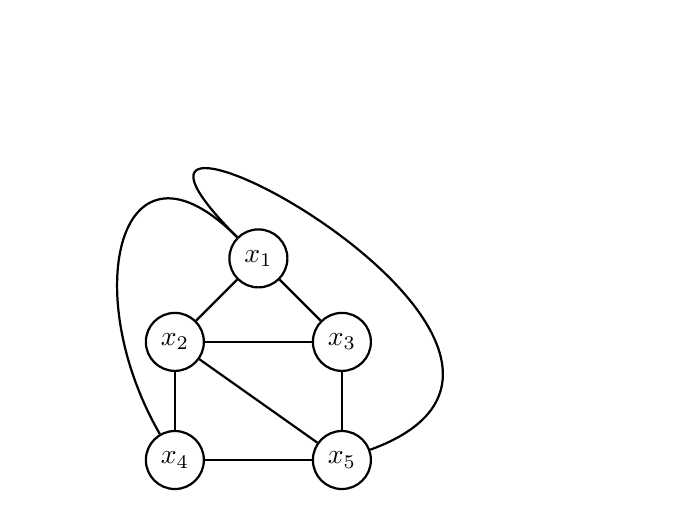
\begin{tikzpicture}[node distance={15mm}, thick, main/.style = {draw, circle}] 
        \node[main] (1) {$x_1$}; 
        \node[main] (2) [below left of=1] {$x_2$};
        \node[main] (3) [below right of=1] {$x_3$}; 
        \node[main] (4) [below of=2] {$x_4$}; 
        \node[main] (5) [below of=3] {$x_5$};
        \draw (1) -- (2);
        \draw (1) -- (3);
        \draw (2) -- (3);
        \draw (2) -- (4);
        \draw (3) -- (5);
        \draw (4) -- (5);
        \draw (2) -- (5);
        \draw (1) to [out=135,in=120,looseness=2] (4); % TODO: beautify
        \draw (1) to [out=135,in=20,looseness=3] (5);
    \end{tikzpicture} 
\end{example}